%------------------------------------------------------------------------------------------------
\chapter{Supersymmetric Quantum Mechanics}
\thispagestyle{empty}
Here the formalism of Hamiltonian 1-dimensional supersymmetric Quantum Mechanics 
is introduced, then its fundamental properties will be stated and proven; in the
end, some applications to 1-dimensional and 3-dimensional potentials will be
explored in detail.
\section{First definitions}
The fundamental structure of supersymmetric Quantum Mechanics is based on two
operators:
\begin{gather*}
\hat A = \frac{\hbar}{\sqrt{2m}}\dv[]{}{x} + W(x)\\
\hat A^\dagger = -\frac{\hbar}{\sqrt{2m}}\dv[]{}{x} + W(x).
\end{gather*}
that will be used to construct two Hamiltonians.
\begin{defn}
The real function $W(x)$ is called \textit{superpotential}.
\end{defn}
\begin{defn}
The self-adjoint operators
\begin{gather}
\hat H_1 := \hat A^\dagger\hat A \label{def:H1}\\
\hat H_2 := \hat A\hat A^\dagger \label{def:H2}
\end{gather}
are called \textit{supersymmetric partners Hamiltonians}, and it is trivial to show that
\begin{gather*}
\hat H_1 = -\frac{\hbar^2}{2m}\dv[2]{}{x} + V_1(x)\\
\hat H_2 = -\frac{\hbar^2}{2m}\dv[2]{}{x} + V_2(x),
\end{gather*}
where 
\begin{gather}
V_1(x) = W^2(x)-\frac{\hbar}{\sqrt{2m}}W'(x)\label{eq:V_1}\\
V_2(x) = W^2(x)+\frac{\hbar}{\sqrt{2m}}W'(x)\label{eq:V_2}.
\end{gather}
\end{defn}
These definitions employ the typical language of supersymmetric theories: its
fundamental algebraic structure will now be briefly introduced.
\newpage
\section{Hints at supersymmetric Algebra}
\label{sec:susy_algebra}
Similarly to classical Hamiltonian mechanics, in Quantum Mechanics every symmetry
is closely related to an operator commuting with the
Hamiltonian of the system: Supersymmetry can also be defined in similar terms.

Given the operators defined earlier, consider the operators

\begin{equation*}
\hat Q = \begin{pmatrix}
    \mathbb{O}&\mathbb{O}\\
    \hat A&\mathbb{O}
\end{pmatrix}\text{,   }
\hat Q^\dagger = \begin{pmatrix}
    \mathbb{O}&\hat A^\dagger\\
    \mathbb{O}&\mathbb{O}
\end{pmatrix}
\label{eq:alg_1}
\end{equation*}
and the Hamiltonian
\begin{equation*}
\hat H := \left\{\hat Q,\hat Q^\dagger\right\}= 
\begin{pmatrix}
    \hat A^\dagger\hat A& \mathbb{O}\\
    \mathbb{O}&\hat A\hat A^\dagger
\end{pmatrix} =
\begin{pmatrix}
    \hat H_1& \mathbb{O}\\
    \mathbb{O}&\hat H_2
\end{pmatrix},
\end{equation*}

The (vector) ground state of $\hat H$ is
$$\psi_0=\begin{pmatrix}
\psi^{(1)}_0\\
\psi^{(2)}_0
\end{pmatrix},
$$
where $\psi^{(i)}_0$ are the ground states of $\hat H_i$.

The definition of the Hamiltonian $\hat H$ is the first property of the
supersymmetric Algebra, the others follow from the definitions of $\hat Q$ and
$\hat H$:
\begin{equation*}
\left[\hat H, \hat Q\right]= \left[\hat H, \hat Q^\dagger\right]=0
\end{equation*}
and 
\begin{equation*}
\left\{\hat Q,\hat Q\right\}=\left\{\hat Q^\dagger,\hat Q^\dagger\right\}=0.
\label{eq:alg_2}
\end{equation*}
\textbf{Note} The symmetry is given by the fact that $\hat Q,\; \hat Q^\dagger$
commute with the Hamiltonian of the system.

To introduce the concept of supersymmetry breaking, some properties of the
partner Hamiltonians need to be considered.

%\begin{defn}
%The conditions (\ref{eq:alg_1}) to (\ref{eq:alg_2}) define a Lie Superalgebra.
%\end{defn}%forse inutile

\COMMENT{
\begin{defn}
Supersymmetry is \textbf{spontaneously broken} if and only if
\begin{equation*}
\hat Q \psi_0 \neq0,\quad\hat Q^\dagger\psi_0\neq0.
\end{equation*}
\label{def:b_algebra}
\end{defn}
\begin{defn}
Supersymmetry is \textbf{unbroken}
if and only if
\begin{equation*}
\hat Q \psi_0 = \hat Q^\dagger\psi_0=0.
\end{equation*}\label{def:unb_algebra}
\end{defn}
These definitions are inspired by the definition of broken symmetries in Quantum
Mechanics.
\newpage}
\section{Fundamental properties of supersymmetric partners}
The most interesting properties of supersymmetric partner Hamiltonians lie in the
relationships between their energy spectra and corresponding eigenstates.

\begin{thm}
Supersymmetric partner Hamiltonians admit only non-negative eigenvalues.
\end{thm}
\textbf{Proof} Consider the Hamiltonians $\hat H_1, \hat H_2$: $\forall\ket{\psi}$ the
quantities
\begin{gather*}
\bra{\psi}\hat H_1\ket{\psi} = \bra{\psi}(\hat A^\dagger\hat A)\ket{\psi} = 
\left|\left| \hat A \ket{\psi} \right|\right|^2\\
\bra{\psi}\hat H_2\ket{\psi} = \bra{\psi}(\hat A\hat A^\dagger)\ket{\psi} = 
\left|\left| \hat A^\dagger \ket{\psi} \right|\right|^2
\end{gather*}
are non-negative, thus proving the statement.\qed\\

In addition to this interesting property, supersymmetric partner Hamiltonians' spectra are
related, due to the fact that they are constructed with the same two operators:
consider the eigenstate $\ket{E^{(1)}}$ for $\hat H_1$ with eigenvalue $E$,
such that
$$\hat H_1 \ket{E^{(1)}} = E \ket{E^{(1)}}.$$
Applying the operator $\hat A$ to both sides yields
$$\hat A\hat H_1\ket{E^{(1)}} = E\hat A\ket{E^{(1)}}.$$
Recalling (\ref{def:H1}) and (\ref{def:H2}),
\textbf{if} $\mathbf{\hat A\ket{E^{(1)}}\neq0}$ (thus $E\neq0$), this is
equivalent to
$$\hat A\hat A^\dagger\hat A\ket{E^{(1)}} = E \hat A \ket{E^{(1)}}
\Rightarrow \hat H_2\hat A \ket{E^{(1)}} =
E\hat A\ket{E^{(1)}}.$$
This shows that the state
\begin{equation}
    \ket{{E^{(2)}}} :=\frac{1}{\sqrt{E}}\hat A\ket{E^{(1)}}
\label{eq:A_use}
\end{equation}
is a normalized eigenstate of $\hat H_2$ with eigenvalue $E$.

Similarly, it can be shown that for an eigenstate $\ket{E^{(2)}}$ of $\hat H_2$,
\textbf{if} $\mathbf{\hat A^\dagger\ket{E^{(2)}}\neq0}$, the state
\begin{equation}
\ket{E^{(1)}} :=\frac{1}{\sqrt{E}}\hat A^\dagger\ket{E^{(2)}}
\label{eq:A+_use}
\end{equation}
is a normalized eigenstate of $\hat H_1$ with eigenvalue $E$.

If, on the other hand, $\hat A \ket{E^{(1)}}=0$ or
$\hat A^\dagger \ket{E^{(2)}}=0$, the eigenvalue of both these eigenstates
must be $E=0$; to see the implications of this condition, it is useful to consider
the energy spectra of $\hat H_1,\hat H_2$ to be discrete, and so from this point
onwards the eigenfunctions and eigenvalues of the Hamiltonians will be denoted as
$$\hat H_i \psi^{(i)}_n = E^{(i)}_n\psi^{(i)}_n.$$
Consider now the case $\hat A \psi_n^{(1)}=0$: this implies $\hat H_1 \psi^{(1)}_n=0$, i.e. that
the wavefunction annihilated by $\hat A$ is the ground state of $\hat H_1$, with eigenvalue
$E^{(1)}_0=0$; this equality yields an analytic expression for the ground state of $\hat H_1$:
\begin{gather*}
\hat A \psi^{(1)}_0 = 0 \iff \frac{\hbar}{\sqrt{2m}}\dv[]{}{x}\psi^{(1)}_0(x) =
W(x)\psi^{(1)}_0 \iff \frac{\dd \psi^{(1)}_0}{\psi^{(1)}_0}=
-\frac{\sqrt{2m}}{\hbar}W(x)
\end{gather*}
\begin{equation}
\psi^{(1)}_0(x)=N\exp\left[-\frac{\sqrt{2m}}{\hbar}\int_{x_0}^{x}\dd y W(y)\right].
\label{eq:ground_state}
\end{equation}
\textbf{Note} For this to be a true ground state wavefunction, it must be
continuous and normalizable: this is true if the integral function
$$f(x) = \int_{x_0}^x \dd y W(y)$$
is continuous and if
$$\lim\limits_{x\to\pm\infty}\frac{f(x)}{\ln(\pm x)}=+\infty:$$
this means that $f$ must increase at $+\infty$ and decrease at $-\infty$, since
$f(x)$ is the integral function of $W(x)$, this implies that
\begin{equation}
\begin{dcases}
      0\leq\lim\limits_{x\to+\infty} W(x) \leq+\infty\\
      -\infty\leq\lim\limits_{x\to-\infty}W(x)\leq 0.
  \end{dcases}
    \label{eq:lim_W}
\end{equation}


If the ground state is known, $\hat A \psi^{(1)}_0=0$ provides an expression for
the superpotential
\begin{equation}
W(x)=-\frac{\hbar}{\sqrt{2m}}\frac{\psi'^{(1)}_0(x)}{\psi^{(1)}_0(x)}.
\label{eq:W_ground}
\end{equation}
These considerations about the ground state can be similarly derived using $\hat H_2$, from
$\hat A^\dagger \psi^{(2)}_0=0$:
\begin{gather*}
\psi^{(2)}_0(x)=N\exp\left[\frac{\sqrt{2m}}{\hbar}\int_{x_0}^{x}\dd y W(y)\right],\\
\lim\limits_{x\to\pm\infty}\frac{f(x)}{\ln(\pm x)}=-\infty\implies\begin{dcases*}
-\infty\leq\lim\limits_{x\to+\infty}W(x)\leq0\\
0\leq\lim\limits_{x\to-\infty}W(x)\leq+\infty
\end{dcases*},\\
W(x)=\frac{\hbar}{\sqrt{2m}}\frac{\psi'^{(2)}_0(x)}{\psi^{(2)}_0(x)}.
\end{gather*}
It is easy to show that these two conditions (and so two $E=0$ ground states) cannot cohexist:
\begin{thm}
Only one of the two ground states of partner Hamiltonians can have eigenvalue $E^{(i)}_0=0$.
\end{thm}

\textbf{Proof (by contradiction)} Suppose both ground states have
$E^{(1)}_0 = E^{(2)}_0=0$: by the previous calculations, their wavefunctions are

$$\begin{aligned}
&\psi^{(1)}_0 = N\exp\left[-f(x)\right]\\
&\psi^{(2)}_0 = N\exp\left[f(x)\right]
\end{aligned}\text{  with } f(x)=\frac{\sqrt{2m}}{\hbar}\int_{x_0}^{x}\dd y W(y)
$$
it is clear that these two wavefunctions cannot be simultaneously normalized, a contradiction.
\qed\\

\textbf{Note} From this point, the superpotential $W(x)$ is chosen so that only the
Hamiltonian $\hat H_1$ can possess a $E=0$ ground state.
\newpage
\begin{defn}
Supersymmetry is \textbf{spontaneously broken} if and only if
\label{def:broken_susy}
\end{defn}
$$\hat A \psi^{(1)}_0 \neq0.$$
\begin{defn}
Supersymmetry is \textbf{unbroken} if and only if
\label{def:unbroken_susy}
\end{defn}
$$\hat A \psi^{(1)}_0=0.$$
\textbf{Note}
Since $\hat A\psi^{(1)}_0=0$ is a necessary condition for
(\ref{eq:lim_W}), if the limits of $W(x)$ do not respect these conditions,
Supersymmetry must be spontaneously broken.\\
If Supersymmetry is spontaneously broken, the limits of $W(x)$ can
have any sign save those described in (\ref{eq:lim_W}) and their counterpart
implied by $\hat A \psi^{(2)}_0=0$: this implies that they must have the same
sign.

Another way to define Supersymmetry breaking is through the operators
$\hat Q,\hat Q^\dagger$ defined in Section \ref{sec:susy_algebra}:
$$\hat Q^\dagger \psi_0 = 0 \iff \psi_0^{(2)}\equiv0 \land
\hat A \psi_0^{(1)} =0\iff
\hat Q \psi_0  =0,
$$
so Supersymmetry is unbroken if and only if 
$$\hat Q \psi_0 =\hat Q^\dagger\psi_0=0$$
which closely resembles the definition of spontaneous symmetry breaking in Quantum
Mechanics.

For both broken and unbroken Supersymmetry, the peculiar property of supersymmetric
partner Hamiltonians is expressed in equations (\ref{eq:A_use}) and (\ref{eq:A+_use}):
for discrete spectra, the ground state will
always be denoted by $n=0$, so the labels of the energy levels will be shifted in case of
unbroken Supersymmetry
$$E^{(2)}_{n} = E^{(1)}_{n+1},\;\forall n = 0,1,2...$$
while the labels remain the same if supersymmetry is broken
$$E^{(2)}_n=E^{(1)}_n\neq0,\;\forall n = 0,1,2...$$
The relationships between the eigenfunctions $\psi^{(i)}_n(x)$ with eigenvalues $E^{(i)}_n\neq0$
are then
\begin{gather}
\psi^{(2)}_n(x)= \frac{1}{\sqrt{E^{(1)}_{n+1}}}\hat A\psi^{(1)}_{n+1}(x) \label{eq:A}\\
\psi^{(1)}_n(x)= \frac{1}{\sqrt{E^{(2)}_{n-1}}}\hat A^\dagger\psi^{(2)}_{n-1}(x) \label{eq:A+}
\end{gather}
This shows that knowing the full energy spectrum and eigenfunctions of one of the partner
Hamiltonians is enough to analytically construct the solutions of the other Hamiltonian, except
at most an $E=0$ ground state: this is the fundamental concept of Supersymmetry that will be used
in this thesis.\\

\begin{figure}[H]
    \centering
    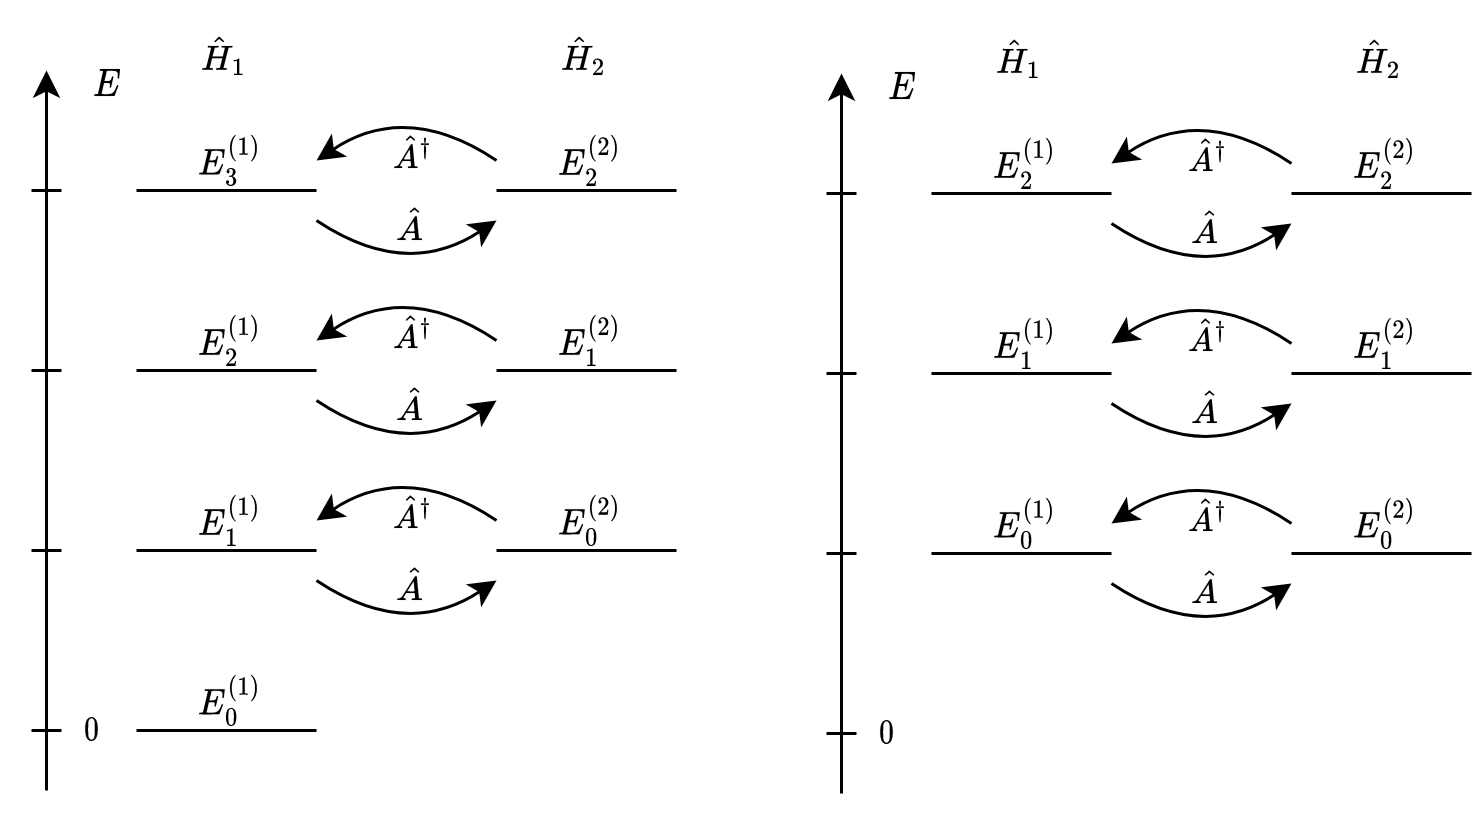
\includegraphics[width = \linewidth]{./SUSY_levels.png}
    \caption{\footnotesize Diagram illustrating the energy levels of $\hat H_1$, $\hat H_2$
    in case of unbroken and broken Supersymmetry (on the left
    and right, respectively) and the operators
    relating their respective eigenfunctions: unbroken Supersymmetry
    is characterized by the $E_0^{(1)}=0$ eigenstate.}
\end{figure}

\textbf{Note} From this point onwards Supersymmetry is considered to be unbroken,
unless otherwise specified.
\section{Example: the infinite square well}
\label{sec:square_well}
Given a simply solvable potential $V_1(x)$, its partner potential $V_2(x)$ can be found
and exactly solved: from this second potential a third ($V_3(x)$) can be derived and so on:
in this section this method is demonstrated beginning from the infinite square well potential.\\

 Consider the potential
$$V_1(x)=\begin{dcases}
-\frac{\pi^2\hbar^2}{2mL^2}&\text{if } 0\leq x\leq L\\
\infty&\text{otherwise}
\end{dcases}.
$$
This is the well known infinite square well potential, with an offset so that its ground state
has $E^{(1)}_0=0$: its energy eigenvalues and corresponding eigenstates are
$$\begin{aligned}
E^{(1)}_n = \frac{\pi^2\hbar^2}{2mL^2}n(n+2),\\
  \psi^{(1)}_n(x)=\sqrt{\frac{2}{L}}\sin\left(\frac{(n+1)\pi x}{L}\right)  
\end{aligned}
\quad\text{with }n=0,1,2,3...$$
Since Supersymmetry is unbroken, the superpotential can be found using equation
(\ref{eq:W_ground}):
$$W(x)= -\frac{\hbar}{\sqrt{2m}}\frac{\psi'^{(1)}_0(x)}{\psi^{(1)}_0(x)} = 
-\frac{\hbar}{\sqrt{2m}}\frac{\frac{\pi}{L}\cos\left(\frac{\pi x}{L}\right)}
{\sin\left(\frac{\pi x}{L}\right)}=-\frac{\hbar\pi}{L\sqrt{2m}}\cot\left(\frac{\pi x}{L}\right)
$$
then, from equation (\ref{eq:V_2}), the partner potential to $V_1(x)$ is
\begin{gather*}
V_2(x) = W^2(x)+\frac{\hbar}{\sqrt{2m}}W'(x)=
\frac{\pi^2\hbar^2}{2mL^2}\left[\cot^2\left(\frac{\pi x}{L}\right) +
\csc^2\left(\frac{\pi x}{L}\right)\right] =\\= \frac{\pi^2\hbar^2}{2mL^2}\left[
2\csc^2\left(\frac{\pi x}{L}\right)-1\right].
\end{gather*}

 Using the properties of superymmetric partner potentials, the energy spectrum of
$\hat H_2$ is readily determined:
$$E^{(2)}_n=E^{(1)}_{n+1}=\frac{\pi^2\hbar^2}{2mL^2}(n+1)(n+3)\quad \text{with }n=0,1,2,3...$$
as said before, the $E=0$ eigenstate exists only for $\hat H_1$.\\

 The eigenfunctions of $\hat H_2$ can be analytically determined with equation
(\ref{eq:A}): the ground state of $\hat H_2$ is
$$\psi^{(2)}_0(x)=\frac{1}{\sqrt{E^{(1)}_1}}\hat A\psi^{(1)}_1 = \frac{1}{\sqrt{E^{(1)}_1}}\left[
\frac{\hbar}{\sqrt{2m}}\dv[]{}{x}+W(x)\right]\psi^{(1)}_1(x)=-2\sqrt{\frac{2}{3L}}\sin^2
\left(\frac{\pi x}{L}\right),$$
with eigenvalue $E^{(2)}_0 = \frac{3\pi^2\hbar^2}{2mL^2}$.\\
 The first excited state of $\hat H_2$ is
$$\psi^{(2)}_1(x)=\frac{1}{\sqrt{E^{(1)}_2}}\hat A\psi^{(1)}_2 = -\frac{2}{\sqrt{L}}
\sin\left(\frac{\pi x}{L}\right)\sin\left(\frac{2\pi x}{L}\right),$$
with eigenvalue $E^{(2)}_1=\frac{8\pi^2\hbar^2}{2mL^2}.$\\

The complete derivation of these wavefunctions can be found in Appendix
\ref{app:square_wave}.\\

This process can be iterated: the potential $V_2(x)$ can be redefined so that
its ground state energy is $0$, a new superpotential $W_2(x)$ can be determined and from this
arises a third potential $V_3(x)$, supersymmetric partner of $V_2(x)-E^{(2)}_0$, with the same
energy spectrum,
except for the $E=0$ eigenvalue; using the new superpotential, the eigenfunctions of $\hat H_3$
can be analytically determined in a similar fashion as before.
%\footnote{forse graficino??}.
\\

This shows that, using the properties of supersymmetric partner potentials, an entire class of
analytically solvable potentials can be constructed starting from an analytically solved problem.

\section{Radial potentials}
The formalism of Supersymmetry can be easily applied to 3-dimensional radial potentials:
as is well known, if a potential $V(r,\vartheta,\varphi)$ is independent of the angular
coordinates, the eigenstates of the Hamiltonian can be factored in
$$\psi_{nlm}(r,\vartheta,\varphi) = \frac{1}{r}R_{nl}(r)Y_{lm}(\vartheta,\varphi),$$
where $Y_{lm}$ are the spherical harmonics and the reduced radial wavefunction $R_{nl}(r)$
satisfies
$$- \dv[2]{R_{nl}}{r}+\left[V(r)+\frac{l(l+1)}{r^2}\right]R_{nl}(r)=ER_{nl}(r),$$
in units where $\hbar=2m=1$.\\
This is a 1-dimensional Schrödinger equation with an effective potential that incorporates
the angular momentum barrier.

\subsection{Example: Oscillator potential}
Consider the superpotential
\begin{equation}
W(r) = \frac{\omega r}{2}-\frac{l+1}{r}:
\label{eq:osc_superpot}
\end{equation}
its associated partner potentials are
\begin{equation}
\begin{dcases}
V_1(r)=\frac{\omega^2r^2}{4}+\frac{l(l+1)}{r^2}-\left(l+\frac{3}{2}\right)\omega\\
V_2(r)=\frac{\omega^2r^2}{4}+\frac{(l+1)(l+2)}{r^2}-\left(l+\frac{1}{2}\right)\omega
\label{eq:osc_pot}
\end{dcases}.
\end{equation}
The potential $V_1(r)$ is the effective potential for the isotropic harmonic oscillator: its
$l$'th partial wave has the $l+1$'th partial wave of the same potential as its supersymmetric
partner. This radial potential will be used later as an example of the advantages of the 
supersymmetric approach.

\section{Transmission and reflection coefficients}
Another implication of the properties of supersymmetric Quantum Mechanics is the relationship
between transmission and reflection coefficients of two partner potentials in scattering
problems: before deriving it, it is necessary to establish the conditions on $W(x)$ that
guarantee the existence of unbound eigenstates.\\

 Consider the usual partner potentials $V_1(x)$ and $V_2(x)$, in units where
$\hbar =2m=1$:
\begin{gather*}
V_1(x)=W^2(x)-W'(x)\\
V_2(x)=W^2(x)+W'(x).
\end{gather*}
The corresponding Hamiltonians $\hat H_1$, $\hat H_2$ admit unbound eigenstates if and only if
$$\lim\limits_{x\to\pm\infty}V_i(x) = L^{(i)}_\pm\in\mathbb{R},$$
and the only way for $V_i(x)$ to have finite limits at infinity is if
$$\lim\limits_{x\to\pm\infty}W(x) = W_\pm\in\mathbb{R}
\iff\lim\limits_{x\to\pm\infty}V_i(x)=W^2_\pm.$$
Under this condition on $W(x)$, the partner Hamiltonians admit unbound eigenstates.

Consider a progressive plane wave of energy $E$ scattering on the potential $V_i(x)$: the
wavefunctions $\psi^{(i)}(x)$ will have limits
$$\begin{dcases*}
      \lim\limits_{x\to-\infty} \psi^{(i)}(x) = e^{ikx}+R_ie^{-ikx}\\
      \lim\limits_{x\to+\infty} \psi^{(i)}(x) = T_ie^{ik'x}
  \end{dcases*}\text{, with}\quad
\begin{aligned}
    k = \sqrt{E-W^2_{-}}\\
    k'= \sqrt{E-W^2_{+}}
\end{aligned},$$
where $R_i$ are the \textit{reflection coefficients} and $T_i$ the \textit{transmission
coefficients} of the two potentials.

 Applying property (\ref{eq:A+}) in the limit $x\to-\infty$ yields
\begin{gather*}
e^{ikx}+R_1e^{-ikx} = N\left[-\dv[]{}{x}e^{ikx}+W_-e^{ikx} + R_2\left(
-\dv[]{}{x}e^{-ikx}+W_-e^{-ikx}\right)\right]=\\
=Ne^{ikx}(-ik+W_-)+Ne^{-ikx}(ik+W_-)R_2:
\end{gather*}
equating the coefficients of the exponentials
\begin{equation}
\begin{dcases*}
R_1=N(W_-+ik)R_2\\
N=\frac{1}{W_--ik}
\end{dcases*} \iff R_1 = \frac{W_-+ik}{W_--ik}R_2.
\label{eq:refl}
\end{equation}
Applying the same property to the limit $x\to+\infty$ gives
$$T_1e^{ik'x} = N\left(-\dv[]{}{x}+W_+\right)e^{ik'x}T_2 = N(W_+-ik')T_2,$$
and it follows that
\begin{gather}
T_1 = \frac{W_+-ik'}{W_--ik}T_2.
\label{eq:trans}
\end{gather}
 These two relations imply
\begin{gather*}
|R_1|^2 = |R_2|^2\\
|T_1|^2 = |T_2|^2,
\end{gather*}
which means the transmission and reflection probabilities are the same for both partner
potentials: this result is important, especially in more than 1 dimension, as it relates the
$S$-matrices of different scattering problems.
\section{Example: Reflectionless potentials}
\label{sec:refl1}
In this section the relationship between the transmission and reflection coefficients of partner
Hamiltonians will be used to construct a family of algebraically solvable potentials, starting
from the free particle, which has reflection coefficient $R=0$.

Consider the superpotential
$$W(x;B)=B\tanh(x)$$
and its partner potentials
\begin{gather*}
    V_1(x;B)=B^2-B(B+1)\cosh^{-2}(x)\\
    V_2(x;B)=B^2-B(B-1)\cosh^{-2}(x).
\end{gather*}
Both potentials have finite limits, because
\begin{gather*}
\lim\limits_{x\to\pm\infty}W(x;B)=\pm B\\
\lim\limits_{x\to\pm\infty}V_i(x;B)=B^2,
\end{gather*}
so they always admit unbound eigenstates with $E\geq B^2$.\\

Consider $B=1$: the superpotential and potentials are
\begin{gather*}
W(x;B=1)=\tanh(x)\\
\begin{dcases*}
    V_1(x;B=1)=1-2\cosh^{-2}(x)\\
V_2(x;B=1)=1
\end{dcases*}
\end{gather*}
It is clear that $\hat H_2(B=1)$ is the Hamiltonian of a free particle, so its transmission and
reflection coefficients are
$$
\begin{dcases*}
T_2(k;B=1)=1\\
R_2(k;B=1)=0.
\end{dcases*}
$$
Then, from equations (\ref{eq:refl}) and (\ref{eq:trans}), it follows that the coefficients for
$H_1$ are
$$
\begin{dcases*}
T_1(k;B=1)=\frac{1-ik}{-1-ik}\\
R_1(k;B=1)=0
\end{dcases*}.
$$
Using (\ref{eq:ground_state}), the ground state wavefunction is
$$\psi^{(1)}_0(x;B=1)=N\exp\left[-\int_{x_0}^{x}\dd y\tanh(y)\right]=N\cosh^{-1}(x)$$
and it is normalizable: from the properties discussed before, this
implies that Supersymmetry is unbroken, so $\hat H_1(B=1)$ admits exactly one bound
state with $E^{(1)}_0(B=1)=0$ and a continuum of unbound states with
$E^{(1)}(B=1)\geq1$.\\

Consider now $B=2$, the two potentials are
$$\begin{dcases*}
    V_1(x;B=2)=4-6\cosh^{-2}(x)\\
V_2(x;B=2)=4-2\cosh^{-2}(x)
\end{dcases*}
$$
and it is clear that $V_2(x;B=2)$ differs from $V_1(x;B=1)$ just by a constant, so its
transmission and reflection coefficients must be the same (and their eigenfunctions are
proportional to one another); using once again equations (\ref{eq:refl}) and (\ref{eq:trans}),
the transmission coefficient of $\hat H_1(B=2)$ is
$$
T_1(k;B=2)=\frac{2-ik}{-2-ik}\frac{1-ik}{-1-ik}
$$
and its ground state wavefunction is
$$\psi^{(1)}_0(B=2)=N\cosh^{-2}(x)$$
so Supersymmetry must again be unbroken and $E^{(1)}_0(B=2)=0$; it is also clear that
$\hat H_2(B=2)$ admits a bound state with $E^{(2)}_0(B=2)=3$ (its ground state), and so does
$\hat H_1(B=2)$: the corresponding eigenfunction is
\begin{gather*}
\psi^{(1)}_1(x;B=2)=\hat A^{\dagger}(B=2)\psi^{(2)}_0(x;B=2)=\\
=\hat A^\dagger(B=2)\psi^{(1)}_0(x;B=1)=N\tanh(x)\cosh^{-1}(x),
\end{gather*}
where the first equality is due to the properties of partner Hamiltonians and the second
is due to the fact that $V_2(B=2) = V_1(B=1)+3$.\\

This process can be iterated: $\forall B=p\in\mathbb{N}$, the potentials $V_2(x;p)$ are
reflectionless (as they differ from $V_1(x;p-1)$ just by a constant and so on),
and so are $V_1(x;p)$, as they are partner potentials; their transmission coefficients are
$$T_1(k;p)=\frac{(p-ik)(p-1-ik)...(1-ik)}{(-p-ik)(-p+1-ik)...(-1-ik)}=
\frac{\Gamma(-p-ik)\Gamma(p+1-ik)}{\Gamma(-ik)\Gamma(1-ik)},$$
their ground state wavefunctions are
$$\psi_0^{(1)}(x;p)=N\exp\left[-p\int_{x_0}^{x}\dd y\tanh(y)\right]=N\cosh^{-p}(x),$$
the first excited state wavefunctions are
$$\psi^{(1)}_1(x;p)=\hat A^\dagger(p)\psi_0^{(1)}(x;p-1)=N\tanh(x)\cosh^{1-p}(x)
$$
and finally the $q$'th excited state ($0<q<p$, as they admit $p$ bound states) can be determined
from the $q-1$'th as
$$\psi^{(1)}_q(x;p) = \hat A^\dagger(p)\psi^{(2)}_{q-1}(x;p)=
\hat A^\dagger(p)\psi^{(1)}_{q-1}(x;p-1),$$
as can be deduced from Figure \ref{fig:reflectionless}.
\begin{figure}[H]
    \centering
    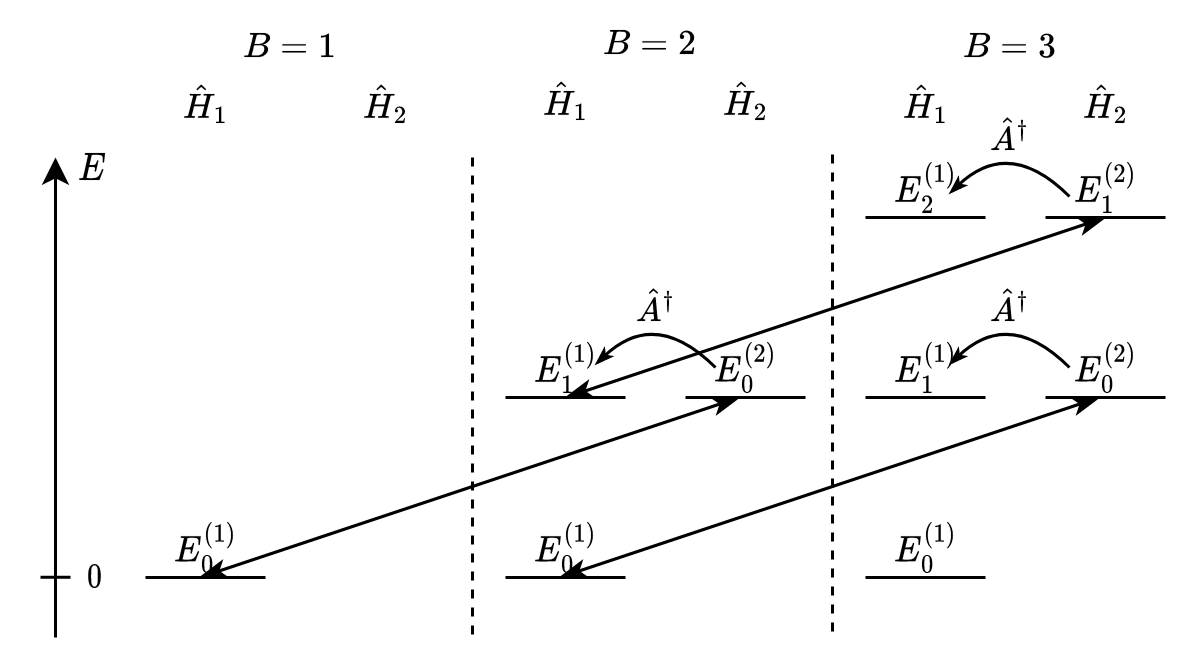
\includegraphics[width = \linewidth]{./reflectionless.png}
    \caption{\small Diagram for the construction of the bound excited states of
    $\hat H_1(B\leq3)$: the equality of the wavefunctions (save normalization) is depicted as a
    double arrow, while the use of the operator $\hat A^\dagger$ with a single arrow.
    The distribution of the levels is not to scale.}
    \label{fig:reflectionless}
\end{figure}

Using the properties of Supersymmetry, it was possible to construct a family of reflectionless
potentials and easily compute their transmission coefficients and bound state wavefunctions, as
they are all related to the free particle Hamiltonian.\\

In this example a more fundamental underlying property that relates the Hamiltonians
$\hat H_i(B)$ to one another, called \textit{shape invariance}, is at work: it will
be discussed more thoroughly in the next chapter.
